\documentclass[a4paper, 12pt]{report}

\usepackage[utf8]{inputenc}
\usepackage[T1]{fontenc}
\usepackage{lmodern}
\usepackage[ngerman]{babel}
\usepackage[margin=3.0cm,top=4cm]{geometry}
\usepackage[]{graphicx}

\usepackage{array}
\usepackage{lastpage}
\usepackage{blindtext} 
\usepackage{amsmath} 
\usepackage{nicefrac}
\usepackage{float}


\newcolumntype{L}[1]{>{\raggedright\let\newline\\\arraybackslash\hspace{0pt}}m{#1}}
\newcolumntype{C}[1]{>{\centering\let\newline\\\arraybackslash\hspace{0pt}}m{#1}}
\newcolumntype{R}[1]{>{\raggedleft\let\newline\\\arraybackslash\hspace{0pt}}m{#1}}


\usepackage{sectsty}
\sectionfont{\fontsize{12}{15}\selectfont}

\renewcommand{\familydefault}{\sfdefault}

\usepackage{fancyhdr}

\pagestyle{fancy}
\fancyhf{}
\fancyhead[L]{Butterworth Hochpass}
\fancyhead[R]{Stefan Urban}
\fancyfoot[R]{Seite \thepage\ von \pageref{LastPage}}
\renewcommand{\headrulewidth}{0.4pt}

%\addtolength{\parskip}{2mm}
\setlength{\parindent}{0pt}


\begin{document}

\section*{Verstärkung}
	\vspace{-0.3cm}
    \begin{minipage}[t]{0.5\textwidth}
	    \[ H(\Omega) = \frac{1}{\sqrt{1 + \left(\frac{1}{\Omega}\right)^{2n}}} \]
    \end{minipage}
    \begin{minipage}[t]{0.5\textwidth}
	    \[ \underline{H}(p) = \frac{1}{\prod_{k=1}^n \left(p - p_{xk}\right)} \]
    \end{minipage}
    
    \vspace{0.5cm}
    
	\begin{minipage}[t]{0.5\textwidth}
  		\section*{Dämpfung}
		\[ a(\Omega) = 10dB \cdot \log{\left(1 + \frac{1}{\Omega^{2n}}\right)} \]
		\[ \Omega(a) = \frac{1}{\sqrt[2n]{10^{a / 10dB} - 1}} \]
	\end{minipage}
	\begin{minipage}[t]{0.5\textwidth}
		 \section*{Asymptoten}
		  \[ a_{\Omega\rightarrow 0,n} = -n \cdot 20dB \cdot \log{(\Omega)} \]
		  \[ a_{\Omega\rightarrow \infty,n} = 0dB \]
	\end{minipage}
	
   	
\section*{Aufwandsabschätzung}
	\vspace{-0.5cm}
   	\begin{minipage}[t]{0.5\textwidth}
		\[ \frac{d}{c} = \sqrt{\frac{10^{a_s/10dB} - 1}{10^{a_p/10dB} - 1}} \]
   	\end{minipage}
   	\begin{minipage}[t]{0.5\textwidth}
   		\vspace{-0.5cm}
		\[ n \ge \frac{\log{\left(\frac{d}{c}\right)}}{\log{\left(\frac{\omega_p}{\omega_s}\right)}} \qquad \qquad n \ge \frac{\log{\left(10^{a_s/10dB}-1\right)}}{2 \cdot \log{\left(\frac{\omega_x}{\omega_s}\right)}}\]
   	\end{minipage}

\section*{Pole und Nullstellen}
	\begin{minipage}[t]{0.6\textwidth}
		\vspace{-5cm}
	    Normierung erfolgt auf Polfrequenz $ \omega_x $!
	    \[ \underline{p}_{xk} = \omega_x \cdot e^{j \cdot (90^{\circ} + \varTheta_{xk})} \qquad k = 1, 2, ... n \]
	    
	    Alle Pole haben gleiche Frequenz:
	    \[ \omega_x = \omega_p \cdot \Omega_p = \omega_s \cdot \Omega_s = \omega_p \cdot \sqrt[2n]{10^{a_p / 10dB} - 1} \]
	    
	    Pole verteilt auf Kreis um Nullpunkt:
	    \[ \varTheta_{xk} = \pi \cdot \left( \frac{2k-1}{2n} \right)  \]
	    
	    Dazugehörige Güten:
	    \[ Q_{xk} = \frac{1}{2 \cdot \sin{\varTheta_{xk}}} \]
	\end{minipage}
   	\begin{minipage}[h]{0.9\textwidth}
   		\vspace{-1cm}
   		\hspace{1cm}
   		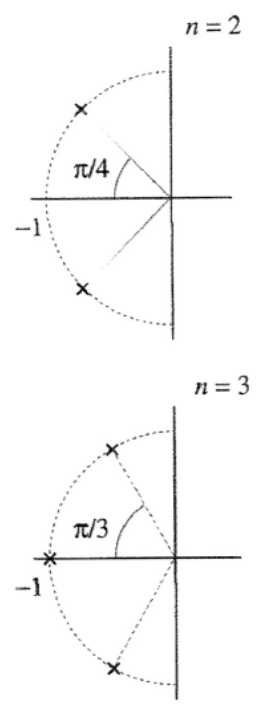
\includegraphics[width=0.3\textwidth]{images/butterworth-pole.png}
   	\end{minipage}
   	
   	
\clearpage
   	
\end{document}
